\documentclass[
size=17pt,
paper=smartboard,
mode=present,
display=slidesnotes,
style=paintings,
nopagebreaks,
blackslide,
fleqn]{powerdot}

% styles: sailor, paintings
% wj capsules prettybox
% mode = handout or present


\usepackage{amsmath,graphicx,color,amsfonts}
\usepackage[brazilian]{babel}
\usepackage[utf8]{inputenc}
\newcommand{\palette}{Europa}


% palettes:
%    - sailor: Sea, River, Wine, Chocolate, Cocktail 
%    - paintings: Syndics, Skater, GoldenGate, Moitessier, PearlEarring, Lamentation, HolyWood, Europa, MayThird, Charon 

\newcommand{\cursopequeno}{EC01008 AOC}
\newcommand{\cursogrande}{\Large EC01008 -- Arquitetura e organização de computadores}



\author{Ronaldo de Freitas Zampolo\\FCT-ITEC-UFPA}
\date{2023-4}


\pdsetup{
   lf = {\cursopequeno},
   rf = {História}, palette = {\palette}, randomdots={false},
   cf = {\theslide}
}


%opening
\title{\cursogrande\\ \vspace{1cm}Destaques da História}

\begin{document}
   \maketitle[randomdots={false}]
   
   \begin{slide}{Agenda}
      \tableofcontents[content=sections]
   \end{slide}
%%%%%%%%%%%%%%%%%%%%%%%%%%%%%%%%%%%%%%%%%%%%%%%%%%%%%%
\section[slide=true]{A primeira geração: válvulas}
\begin{slide}[toc=]{Válvulas}
	\twocolumn{
		\begin{itemize}
			\item Elementos de lógica digital e memória
			\item Alta dissipação de calor
			\item Dimensões grandes
			\item Baixa durabilidade
		\end{itemize}}
		{
		\begin{center}
			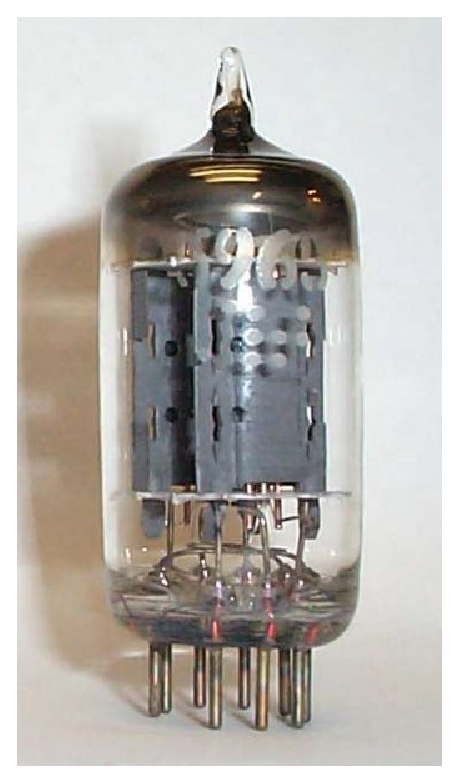
\includegraphics[width=0.6\textwidth]{figs/VacuumTube1}  
		\end{center}
		}
\end{slide}

\begin{slide}[toc=]{ENIAC - generalidades}
   \begin{itemize}
      \item ENIAC: Electronic Numerical Integrator And Computer
      \item Foi o primeiro computador eletrônico de propósito geral construído
      \item Projeto e coordenação: 
      \begin{itemize}
         \item John Adam Presper ``Pres'' Eckert Jr. (engenheiro eletricista, Filadélfia, 9/abr/1919 - Bryn Mawr, 3/jun/1995)
         \item John Mauchly  (físico, Cincinatti, 30/ago/1907 - Ambler, 8/jan/1980)
      \end{itemize}
      \item Local: Universidade da Pensilvânia
      \item Quando: 1943 - 1946 (projeto e construção); usado até 1955
      \item Objetivo: Tabelas de trajetória para armas
   \end{itemize}
\end{slide}
\begin{note}{Universidade da Pensilvânia}
   \begin{itemize}
      \item Localização: Philadelphia, \textbf{Pensilvânia}, EUA
      \begin{center}
         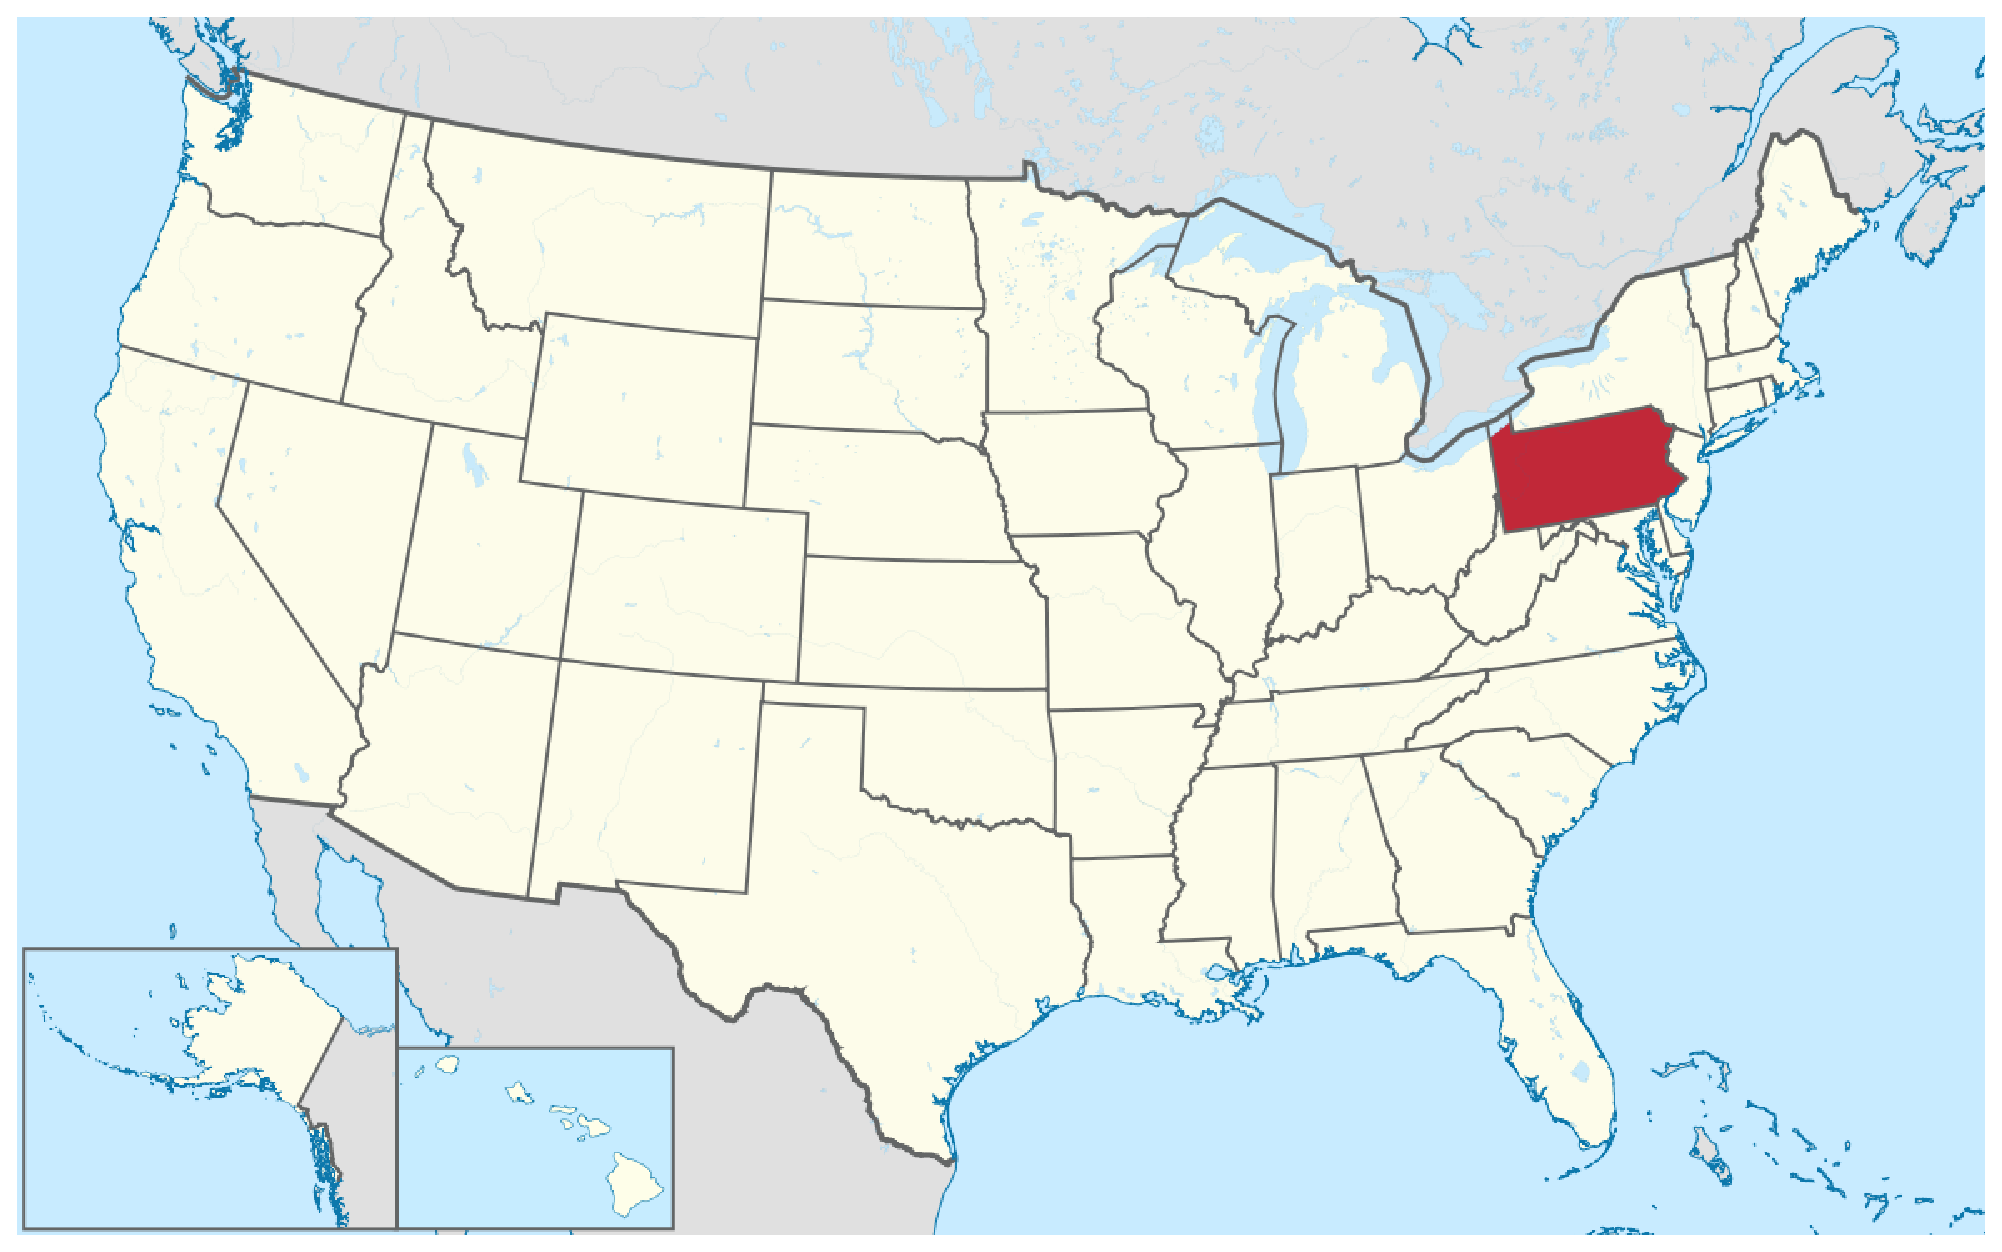
\includegraphics[width=0.5\textwidth]{figs/Pennsylvania_in_United_States.eps}
      \end{center}
      \item Fundada por Benjamin Franklin (17/jan/1706 - 17/abr/1790) 
      \item É a quarta mais antiga instituição de ensino superior (1749) e tida como a primeira universidade dos Estados Unidos 
   \end{itemize}
\end{note}

\begin{slide}[toc=]{ENIAC - características}
   \begin{itemize}
      \item Operação em base decimal (não binário)
      \item 17 468 válvulas, 7 200 diodos a cristal, 1 500 relés, 70 000 resistores, 10 000 capacitores e perto de  5 milhões de junções soldadas à mão !!!
      \item 20 acumuladores de 10 dígitos
      \item Programado manualmente por chaves
      \item 30 toneladas
      \item 167 metros quadrados
      \item 140 kW de potência
      \item 5 000 adições por segundo.
   \end{itemize}
\end{slide}
\begin{note}{Programando o ENIAC}
   Três programadoras do ENIAC em ação...\\
   \begin{center}
      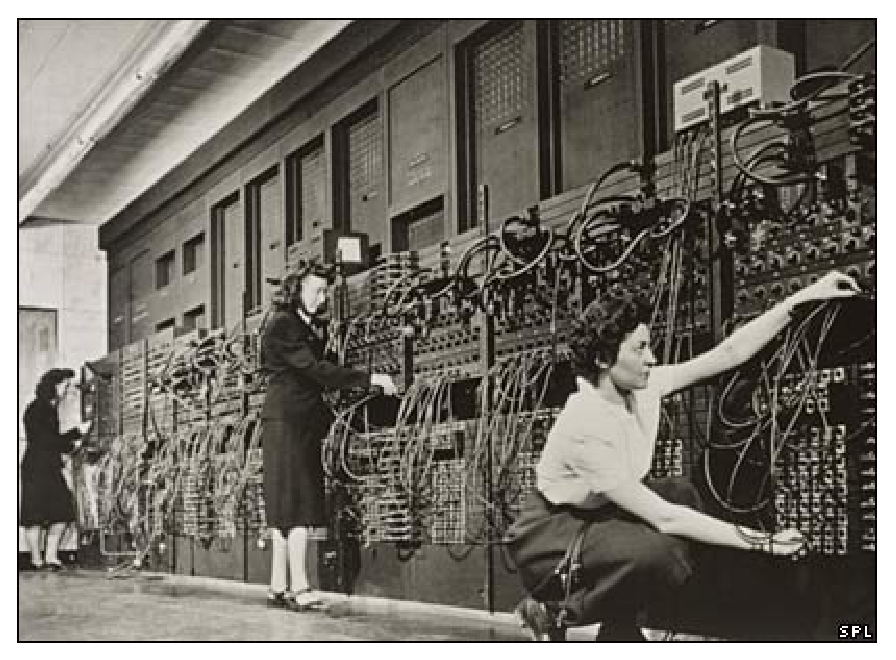
\includegraphics[width=0.6\textwidth]{figs/eniac.eps}  
   \end{center}
\end{note}

%%%%%%%%%%%%%%%%%%%%%%%%%%%%%%%%%%%%%%%%%%%%%%%%%%%%%%%%

\begin{slide}[toc=]{Arquitetura de Von Neumann}
\begin{itemize}
	\item Conceito de programa armazenado (Neumann e Turing desenvolveram o conceito na mesma época)
	\item Memória principal armazenando programas e dados
	\item ALU operando sobre dados binários
	\item Unidade de controle
	\item Equipamento de entrada e saída
\end{itemize}
\end{slide}

\begin{slide}[toc=]{Arquitetura de Von Neumann}
\begin{center}
   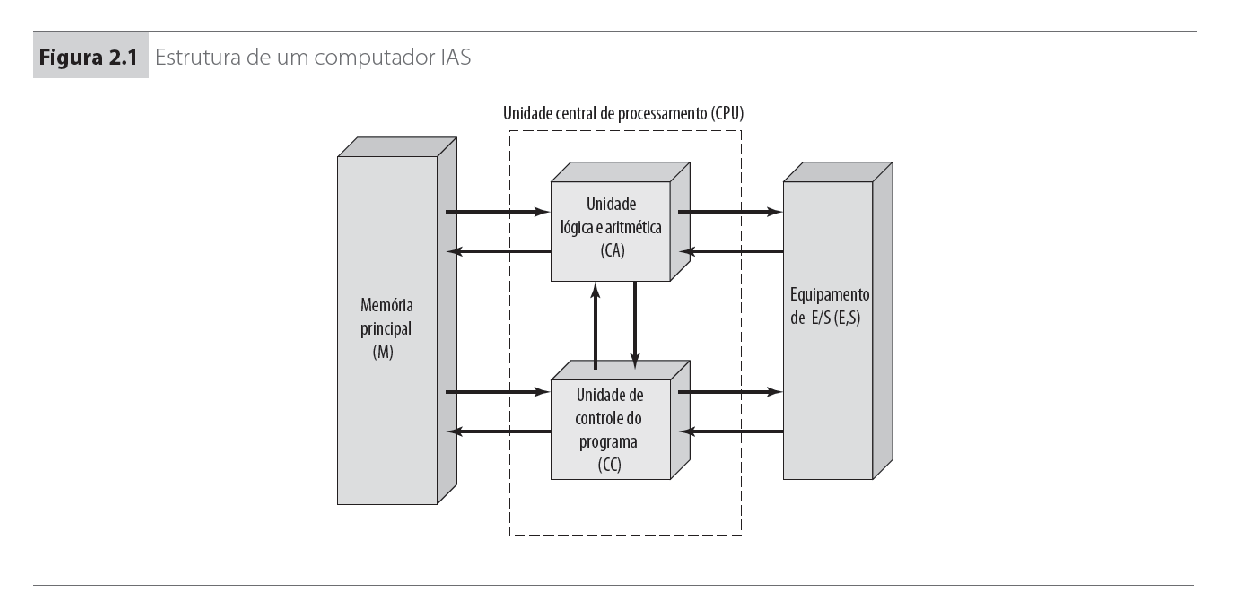
\includegraphics[width=1.0\textwidth]{figs/vneumann} 
\end{center}
\end{slide}

\begin{slide}[toc=]{Máquina IAS - generalidades}
\begin{itemize}
   \item IAS: Institute os Advanced Studies (Princeton, Nova Jersey, EUA)
   \item John von Neumann (28/dez/1903 - 8/fev/1957)
   \item Período de construção: 1946 - 1952
   \begin{center}
      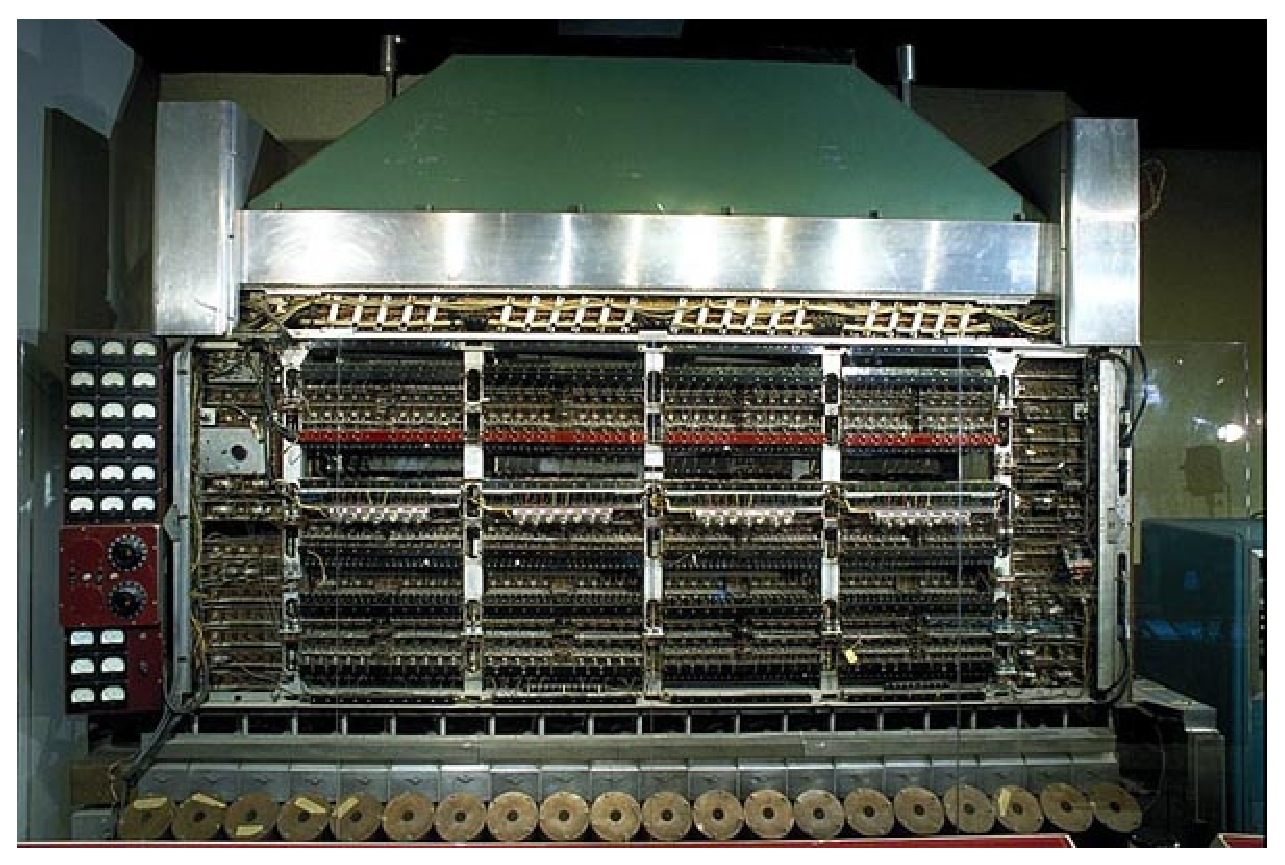
\includegraphics[width=0.60\textwidth]{figs/iasl} 
   \end{center}
\end{itemize}
\end{slide}

\begin{slide}[toc=]{Máquina IAS - características}
\begin{itemize}
   \item Memória: 4096 ``palavras'' de 40 bits
   \item Cada palavra pode ser:
   \begin{itemize}
	   \item Número binário (1 bit para sinal, 39 para magnitude)
	   \item Duas instruções de 20 bits
      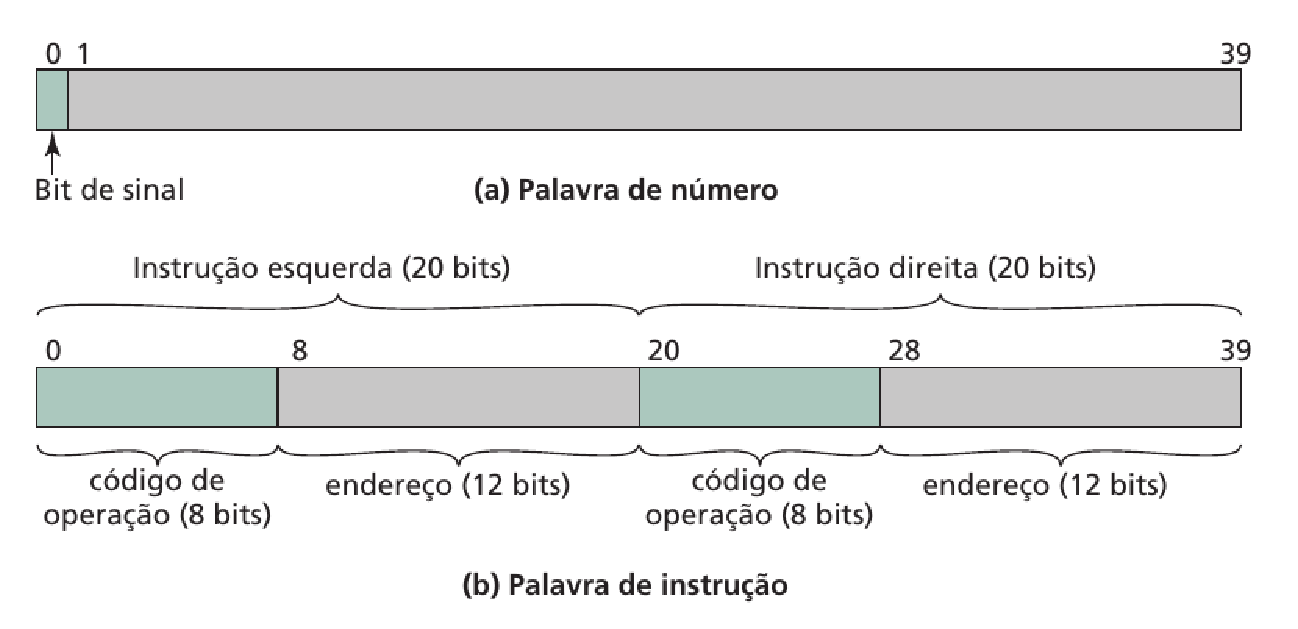
\includegraphics[width=0.8\textwidth]{figs/iasmem}
   \end{itemize}
\end{itemize}
\end{slide}

\begin{slide}[toc=]{Máquina IAS - diagrama}
\begin{center}
   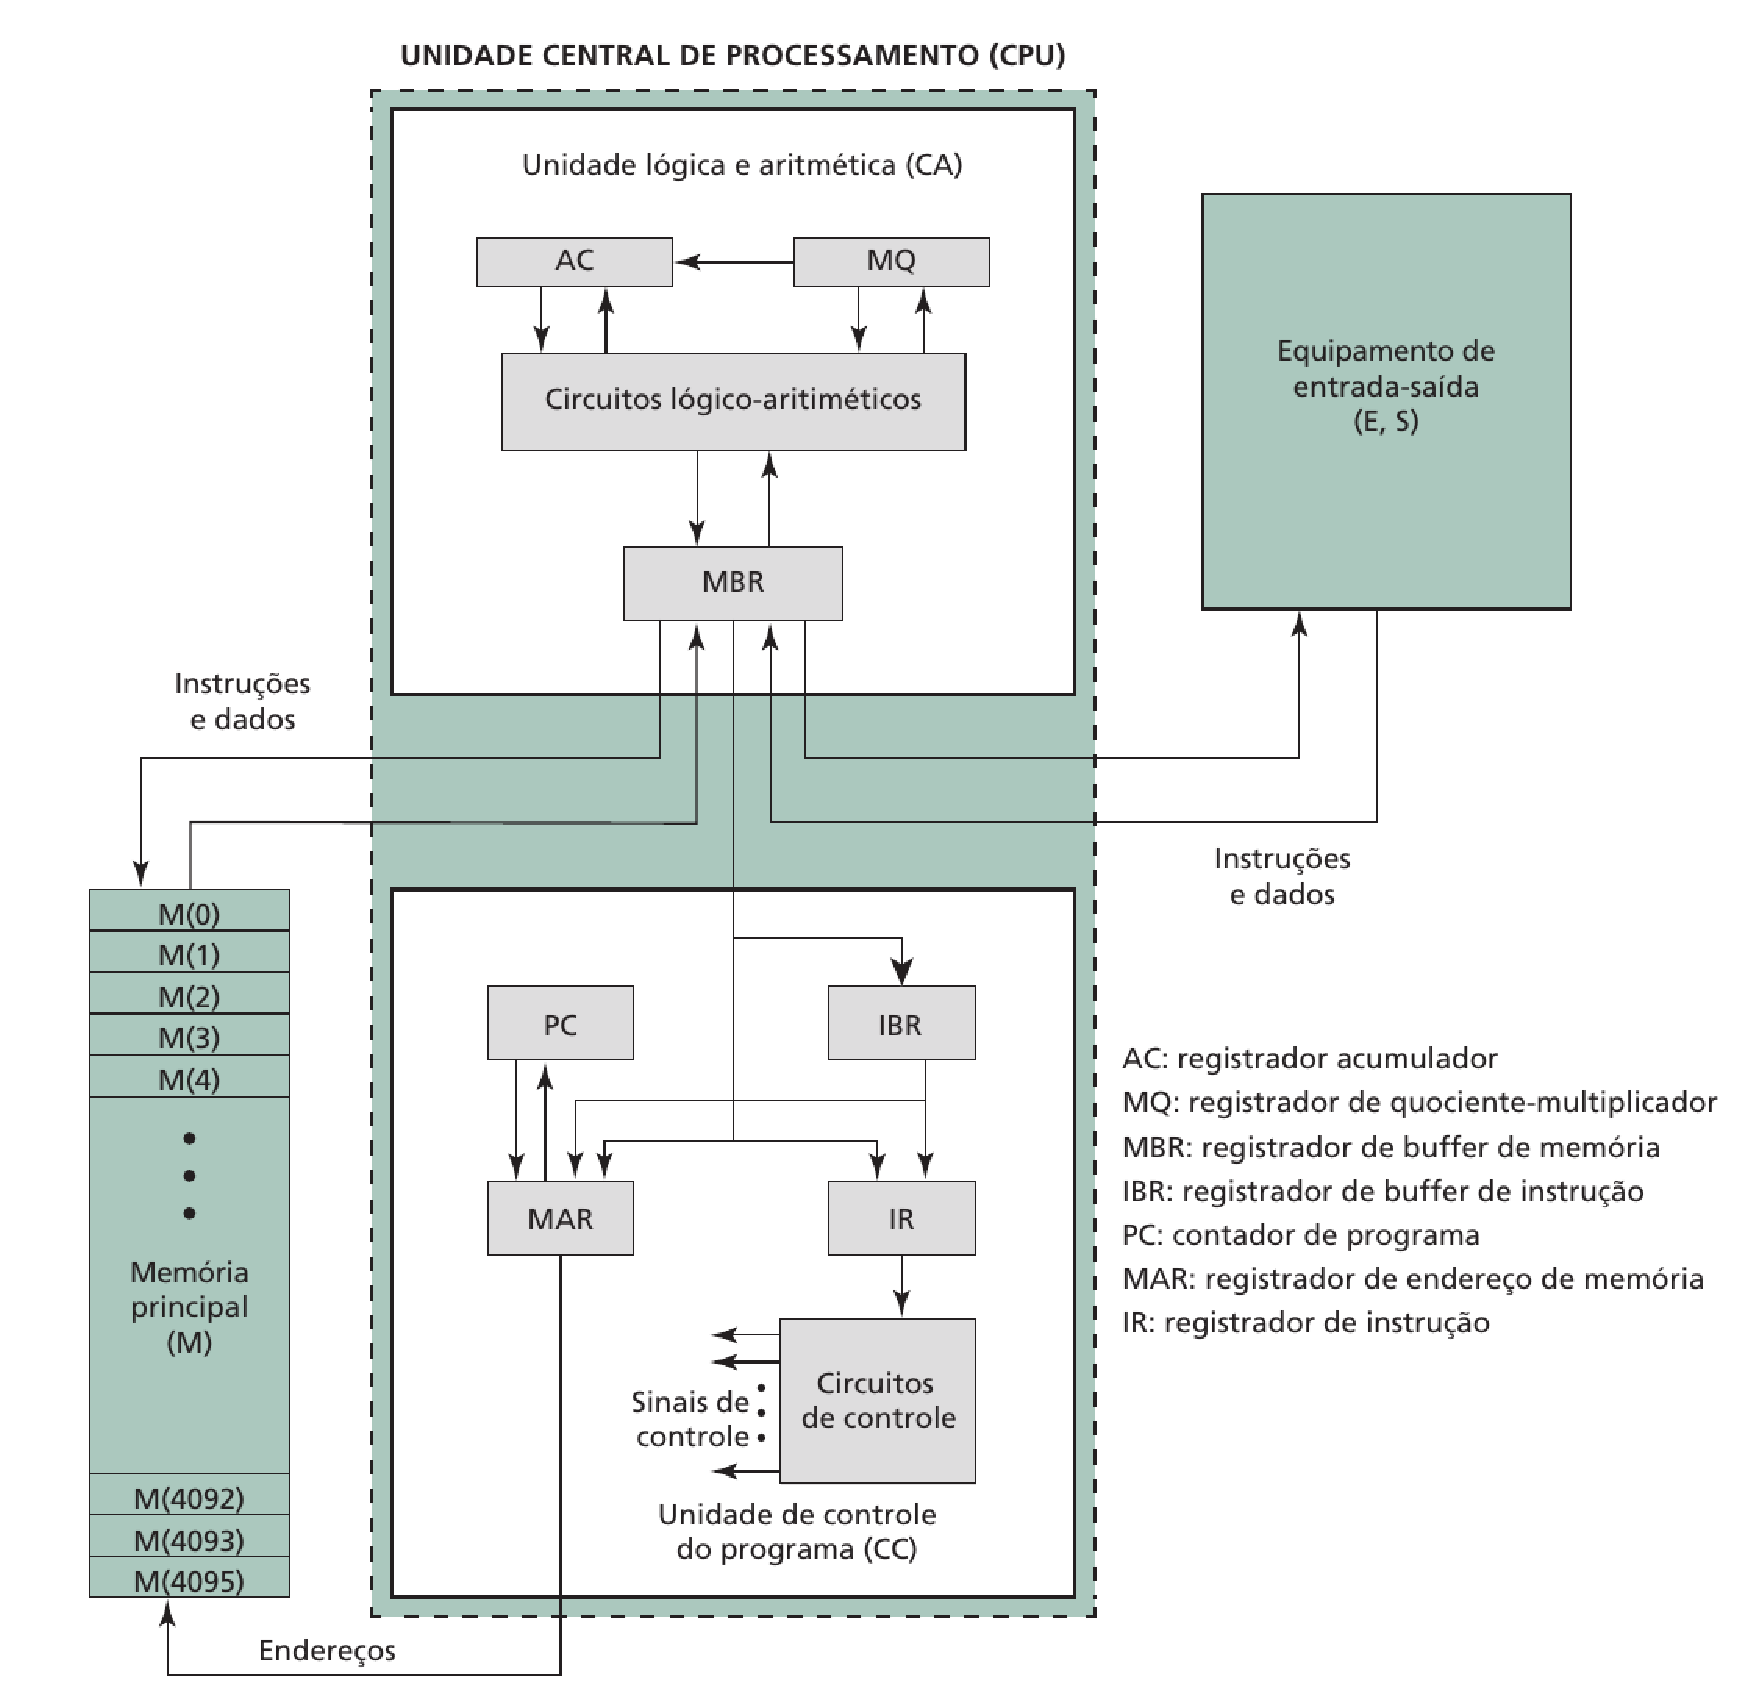
\includegraphics[height=0.80\textheight]{figs/ias2} 
\end{center}
\end{slide}

\begin{slide}[toc=]{Máquina IAS - registradores}
\begin{itemize}
	\item \textbf{Registrador de buffer de memória (MBR, memory buffer register):} contém uma palavra a ser enviada (memória ou E/S) ou uma palavra recebida (da memória ou E/S).
	\item \textbf{Registrador de endereço de memória (MAR, memory address register):} especifica um endereço de memória para palavra que será lida da ou escrita na memória.
	\item \textbf{Registrador de instruções (IR, instrction register):} contém 8 bits referenta ao código de operação (opcode) sendo executado.
	\item \textbf{Registrador de buffer de instruções (IBR, instruction buffer register):} armazena temporariamente a instrução do lado direito.
	\item \textbf{Contador de programa (PC, program counter):} contém o endereço do próximo par de instruções a ser lido da memória.
	\item \textbf{Acumulador (AC), Quociente-multiplicador (MQ, multiplier quotient):} registradores usados para reter temporariamente operandos e resultados da ULA.
\end{itemize}
\end{slide}


\begin{slide}[toc=]{Máquina IAS - fluxograma de operação}
	\begin{itemize}
		\item Ciclo de instrução: ciclo de busca (fetch) + ciclo de execução
	\end{itemize}
\begin{center}
   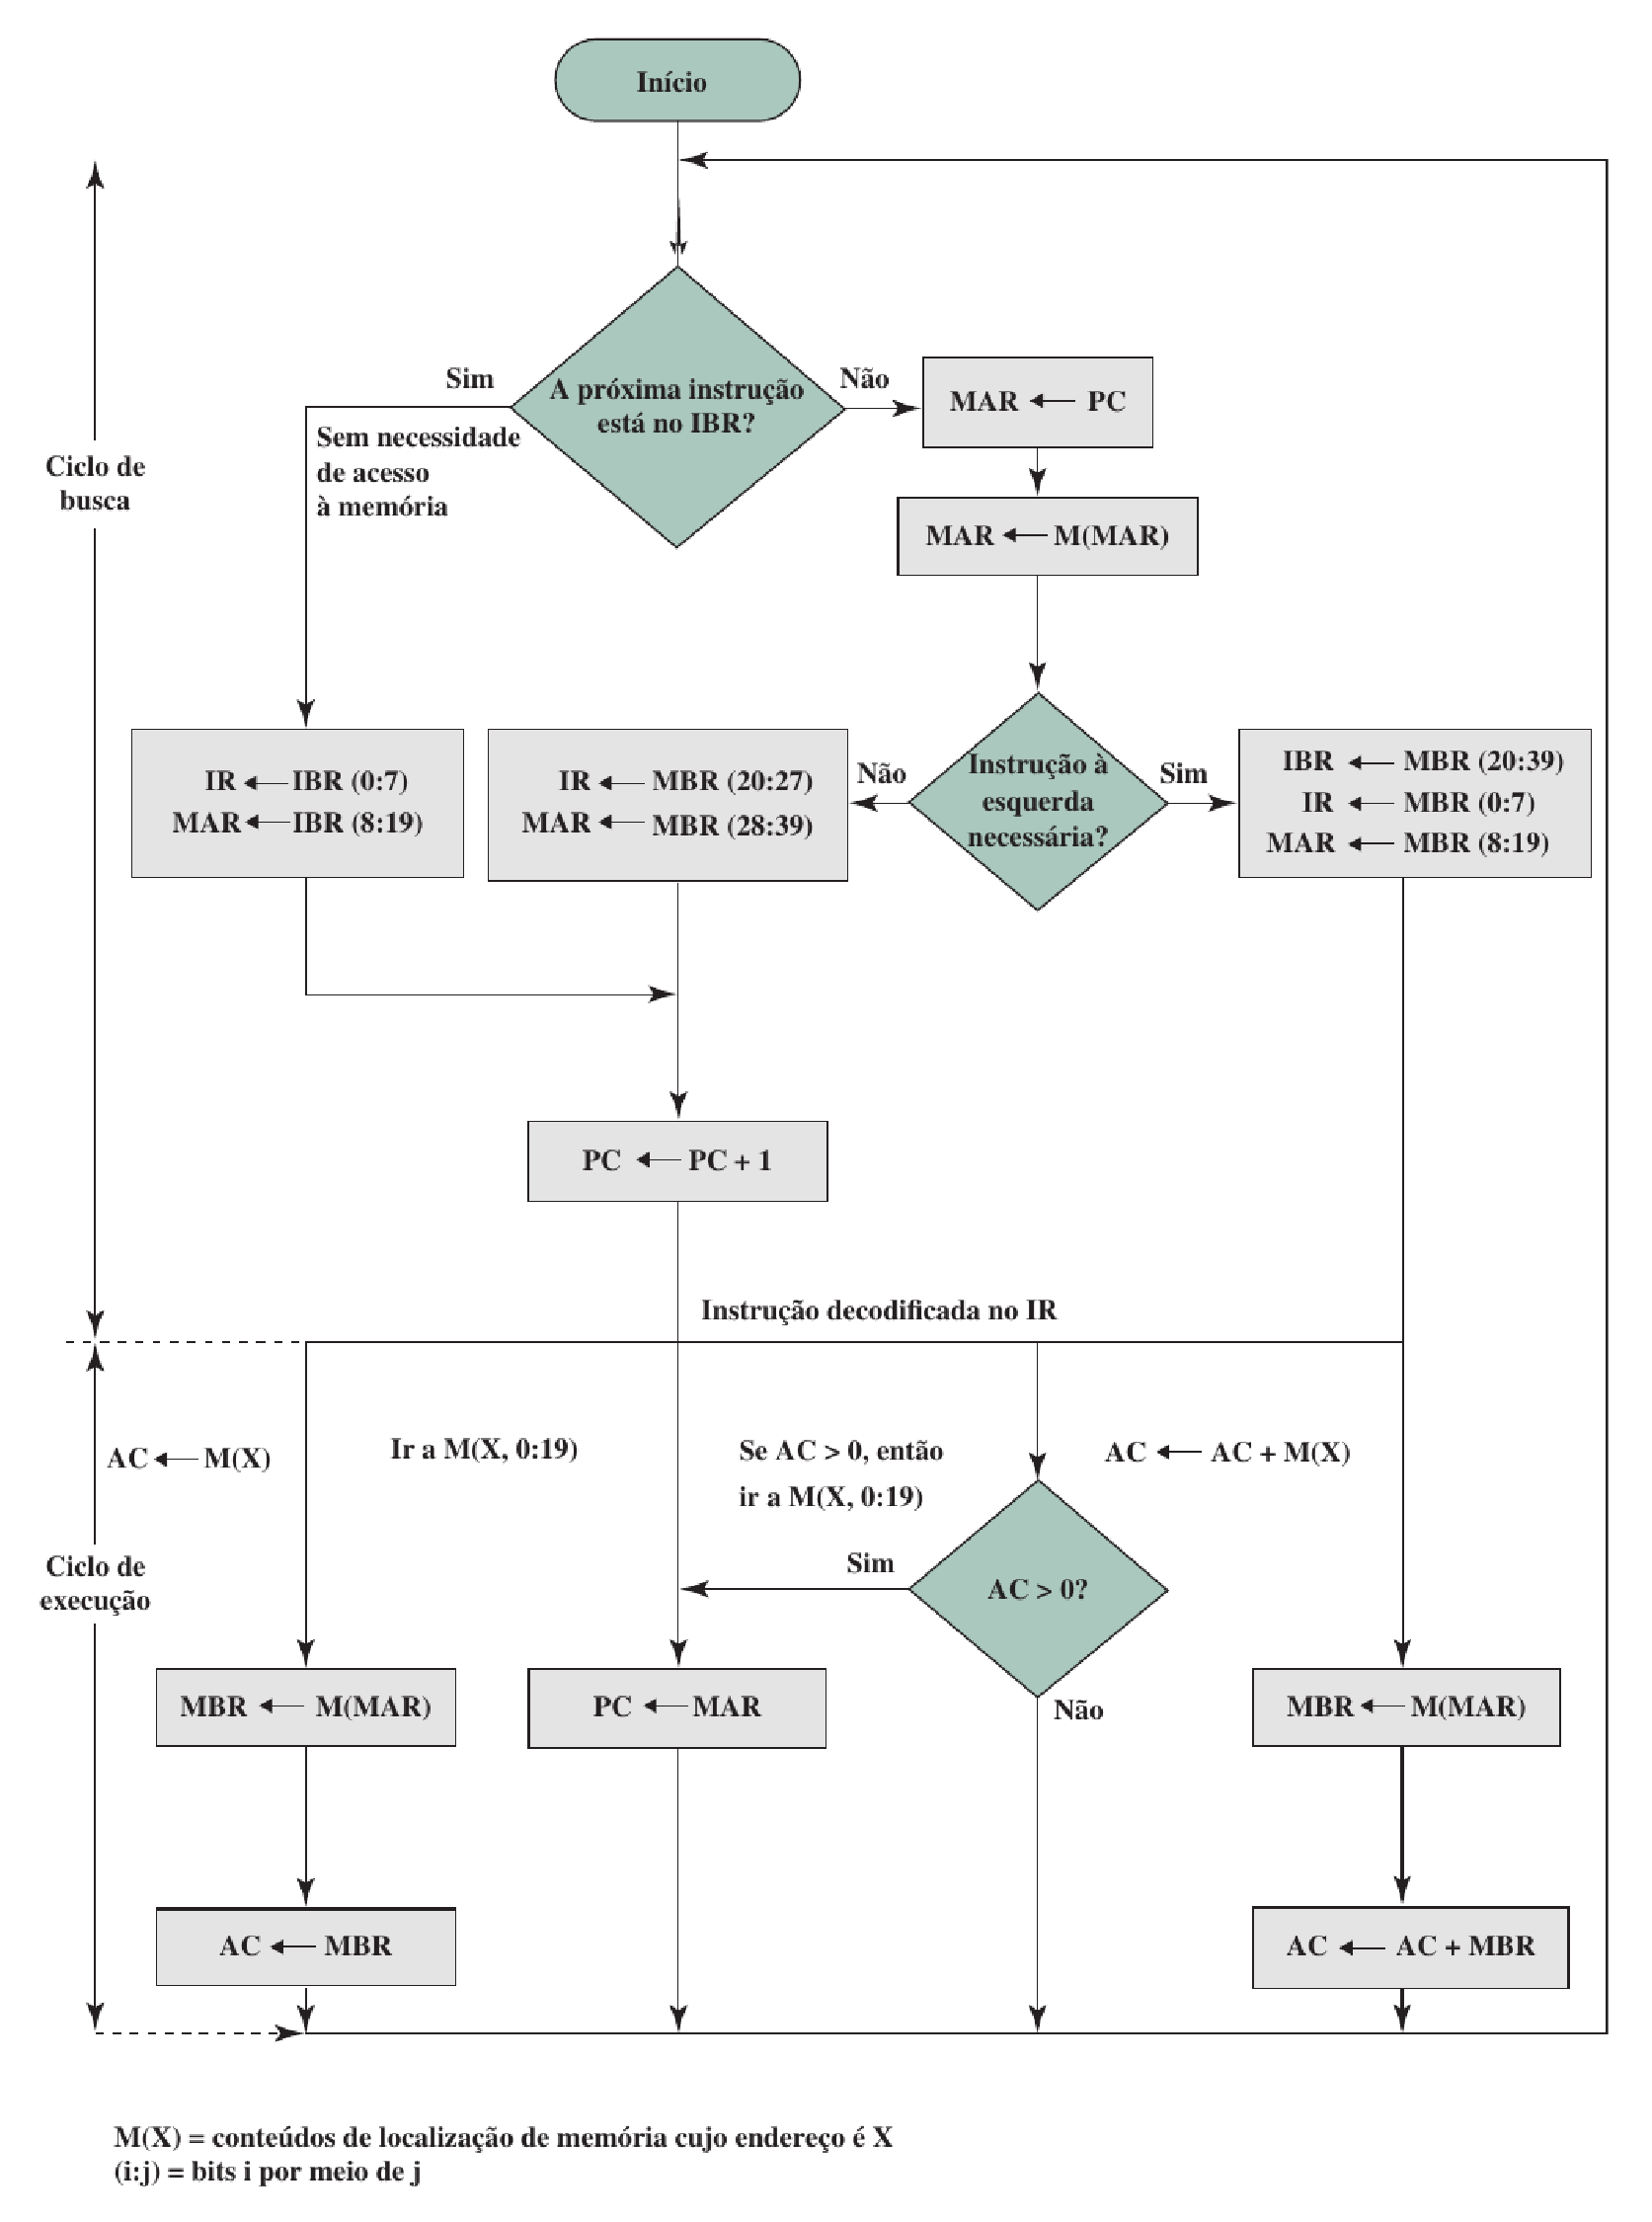
\includegraphics[height=0.70\textheight]{figs/iasfluxopar} 
\end{center}
\end{slide}

\begin{slide}[toc=]{Máquina IAS - instruções}
\begin{center}
   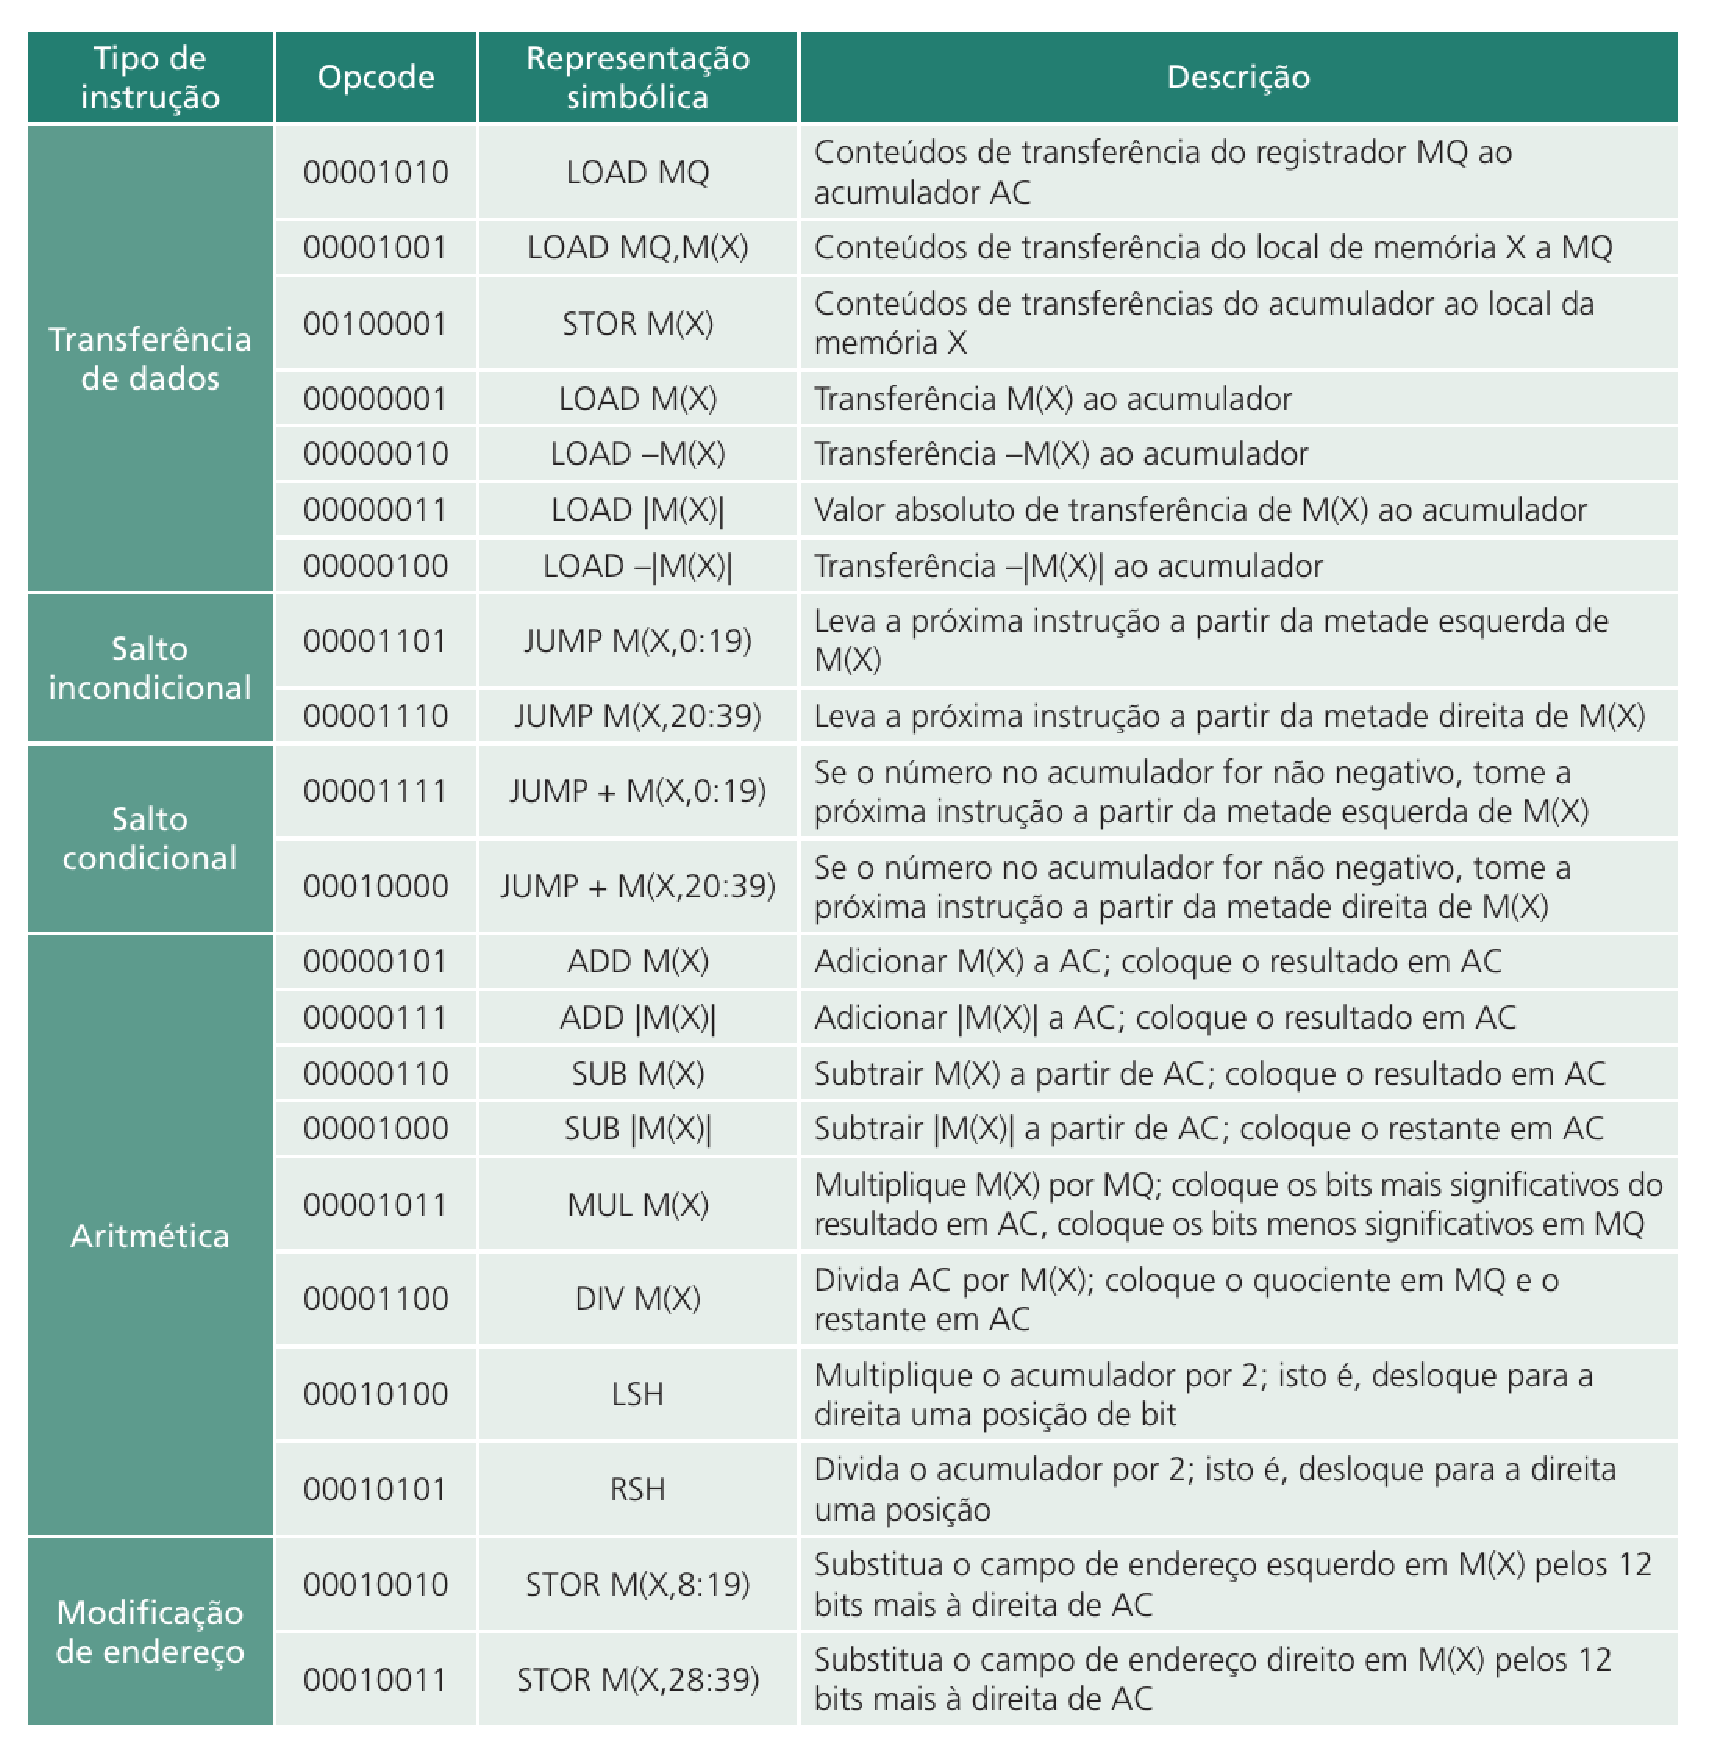
\includegraphics[height=0.8\textheight]{figs/iasinstrucoes} 
\end{center}
\end{slide}

\section[slide=true]{A segunda geração: transistores}
\begin{slide}[toc=]{Transistor}
	\twocolumn{
		\begin{itemize}
			\item Inventado em 1947 nos Bell Labs (Bardeen, Shockley, e Brattain)
			\item Elementos de lógica digital e memória
			\item Menor custo
			\item Menores dimensões 
			\item Menor geração de calor
			\item Encapsulamento mais resistente
		\end{itemize}
		\begin{center}
			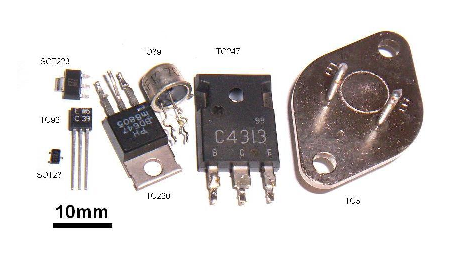
\includegraphics[width=0.9\textwidth]{figs/Transbauformen}  
		\end{center}}
		{
		\begin{center}
			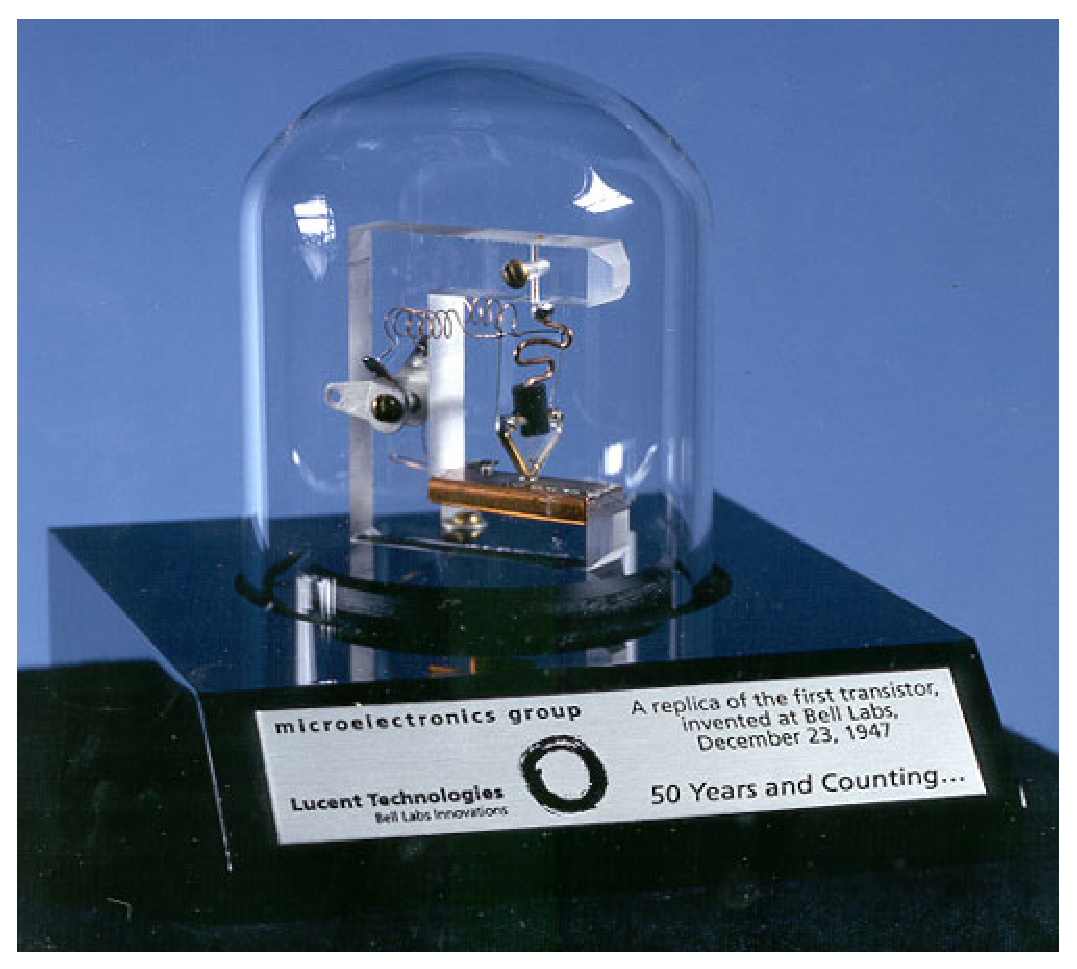
\includegraphics[width=0.8\textwidth]{figs/Replica-of-first-transistor}  
		\end{center}
		}
\end{slide}

%\section[slide=true]{Famílias de computadores}
\begin{slide}[toc=]{IBM série 700/7000}
Máquinas da primeira (válvula) e segunda (transistor) gerações
\begin{center}
   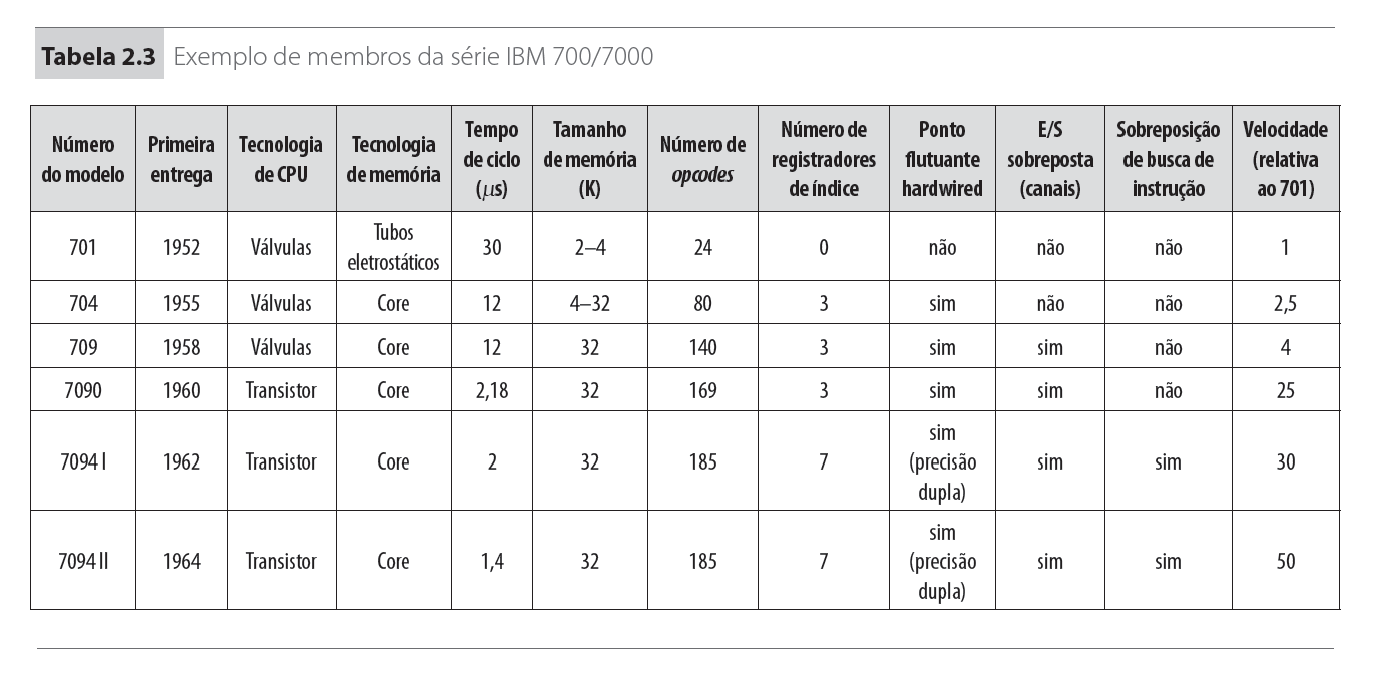
\includegraphics[width=0.99\textwidth]{figs/ibm700} 
\end{center}
\end{slide}

\begin{slide}[toc=]{Configuração do IBM 7094}
	\twocolumn{
		\begin{itemize}
			\item Registrador de backup de instruções: busca antecipada de instruções
			\item Canais de dados: 
				\begin{itemize}
					\item Instruções de E/S na memória principal
					\item Processador principal inicia E/S
					\item Processador de propósito especial no canal de dados: responsável pela execução das instruções de E/S
				\end{itemize}
			\item Multiplexador: regula acesso à memória
		\end{itemize}
		}
		{
		\begin{center}
			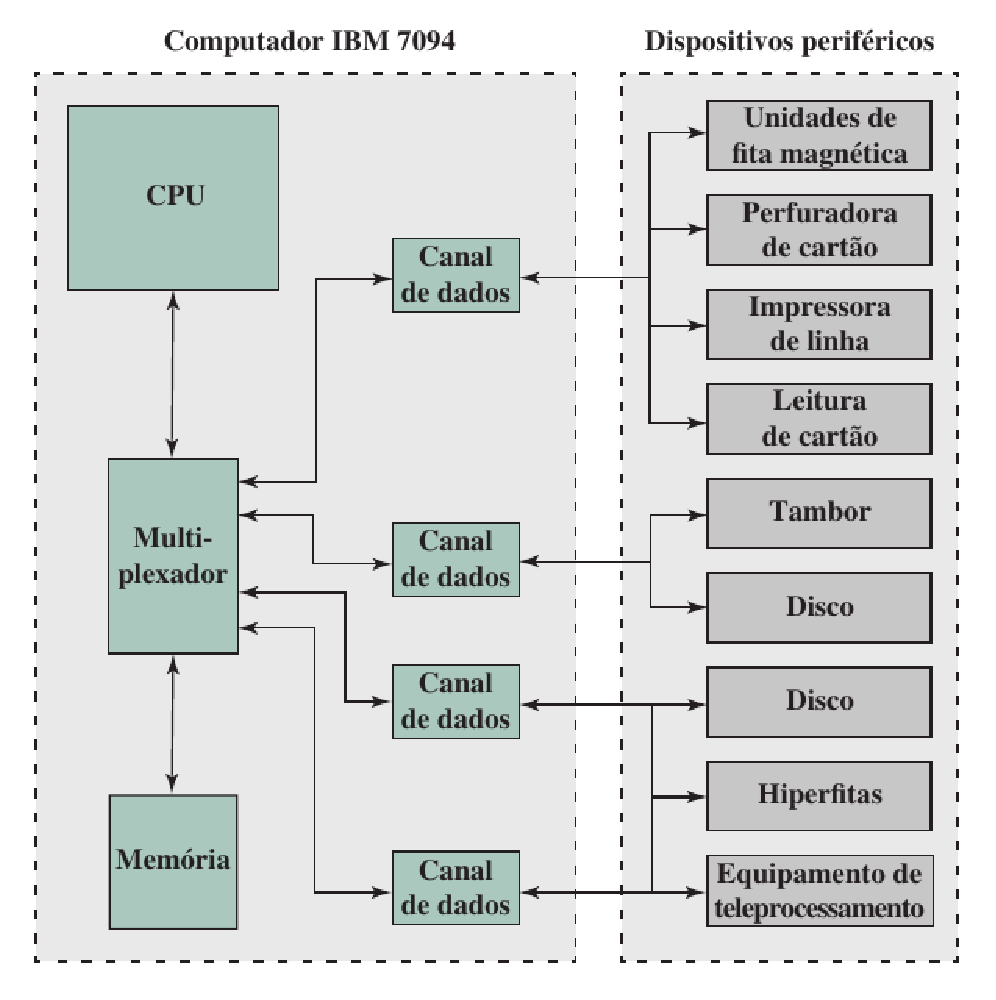
\includegraphics[width=0.99\textwidth]{figs/ibm7094b} 
		\end{center}
		}
\end{slide}


\section[slide=true]{A terceira geração: circuitos integrados}
\begin{slide}[toc=]{Elementos fundamentais em um computador}
	\begin{itemize}
		\item Portas lógicas:
			\begin{itemize}
				\item Entrada/Saída
				\item Linha de ativação (ON/OFF)
			\end{itemize}
		\item Células de memória:
			\begin{itemize}
				\item Entrada/Saída
				\item Linhas para indicação de tipo de operação (Leitura/Escrita)
			\end{itemize}
	\end{itemize}
	\begin{center}
		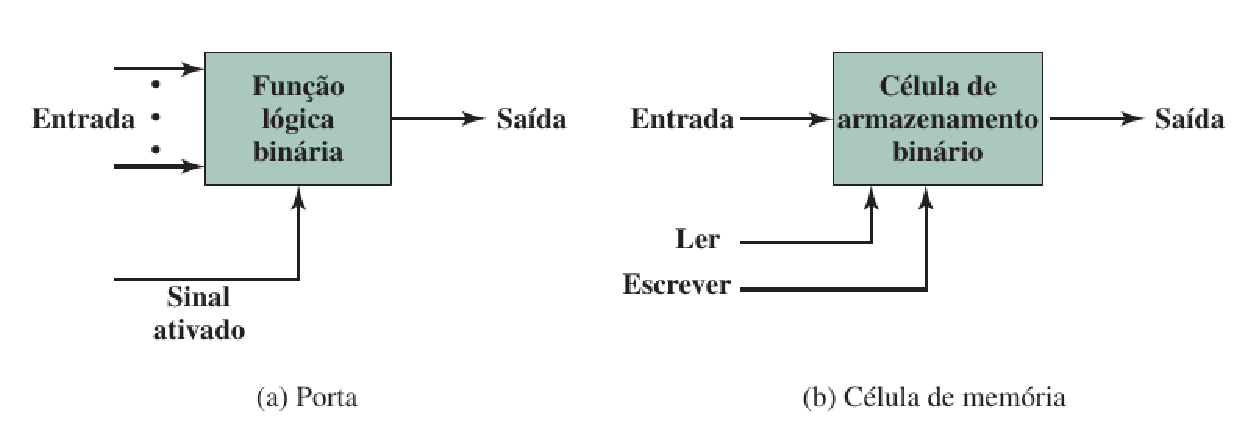
\includegraphics[width=0.8\textwidth]{figs/elementos-fundamentais}
	\end{center}
\end{slide}

\begin{slide}[toc=]{Distinção entre wafer, chip e portas}
	O processo de fabricação permite a produção de vários \emph{chips} em um mesmo \emph{wafer}. Cada \emph{chip}, por sua vez, é composto por um número muito grande de portas lógicas interconectadas.

	\begin{center}
		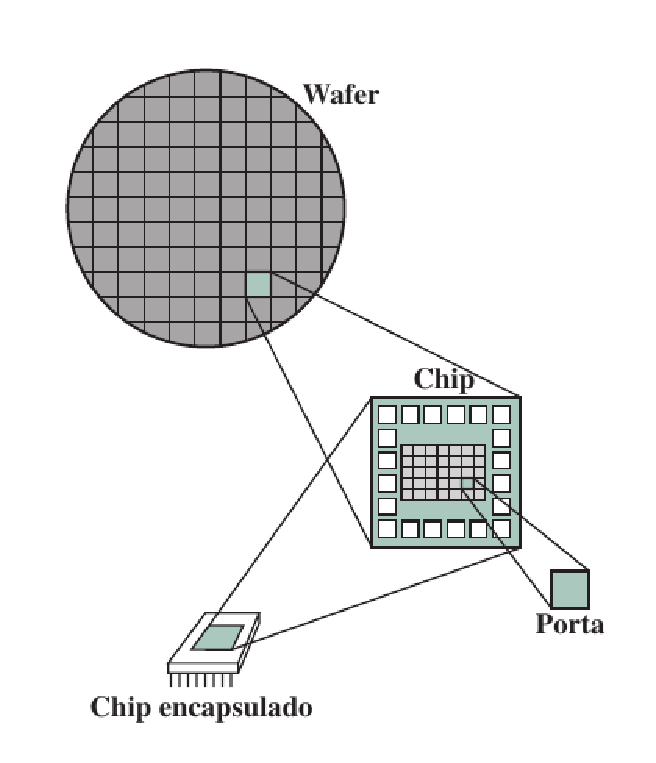
\includegraphics[width=0.35\textwidth]{figs/wafer-chip-porta}
	\end{center}
\end{slide}

\begin{slide}[toc=]{Lei de Moore}
\begin{itemize}
   \item Gordon Earle Moore (3/jan/1929): químico, co-fundador da Intel Corporation
   \item A capacidade de integração dobra a cada dezoito meses
   \item Consequências da Lei de Moore
	   \begin{itemize}
		   \item O custo do chip permaneceu inalterado ao logo do período de rápido aumento de densidade. Ou seja, circuitos caíram de preço.
		   \item Caminhos de condução de dados mais curtos, aumentando a velocidade de operação.
		   \item Computadores ficaram menores e mais portáteis.
		   \item Redução do consumo de energia.
	           \item Conexões no chip são mais confiáveis que conexões externas.
	   \end{itemize}
   \item \footnotesize{``The complexity for minimum component costs has increased at a rate of roughly a factor of two per year... Certainly over the short term this rate can be expected to continue, if not to increase. Over the longer term, the rate of increase is a bit more uncertain, although there is no reason to believe it will not remain nearly constant for at least 10 years. That means by 1975, the number of components per integrated circuit for minimum cost will be 65,000. I believe that such a large circuit can be built on a single wafer.''\\(\emph{Cramming more components onto integrated circuits}, Electronics Magazine 19 April 1965)}
\end{itemize}
\end{slide}

%\begin{slide}[toc=]{Lei de Moore}
%\begin{center}
%   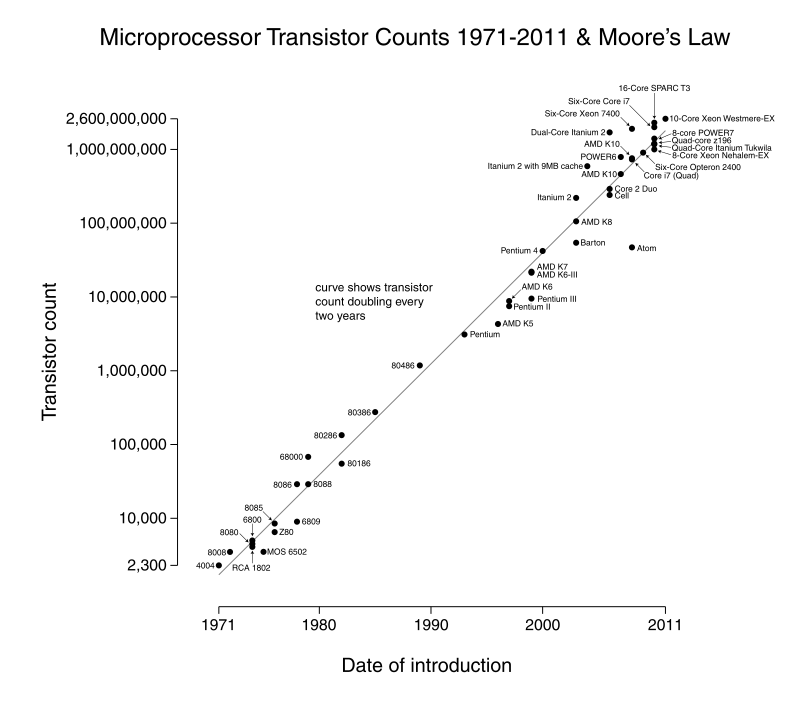
\includegraphics[width=0.60\textwidth]{figs/Transistor_Count_and_Moore's_Law_-_2011} 
%\end{center}
%\end{slide}

\begin{slide}[toc=]{Lei de Moore}
	Contagem de transistores em circuitos integrados
\begin{center}
   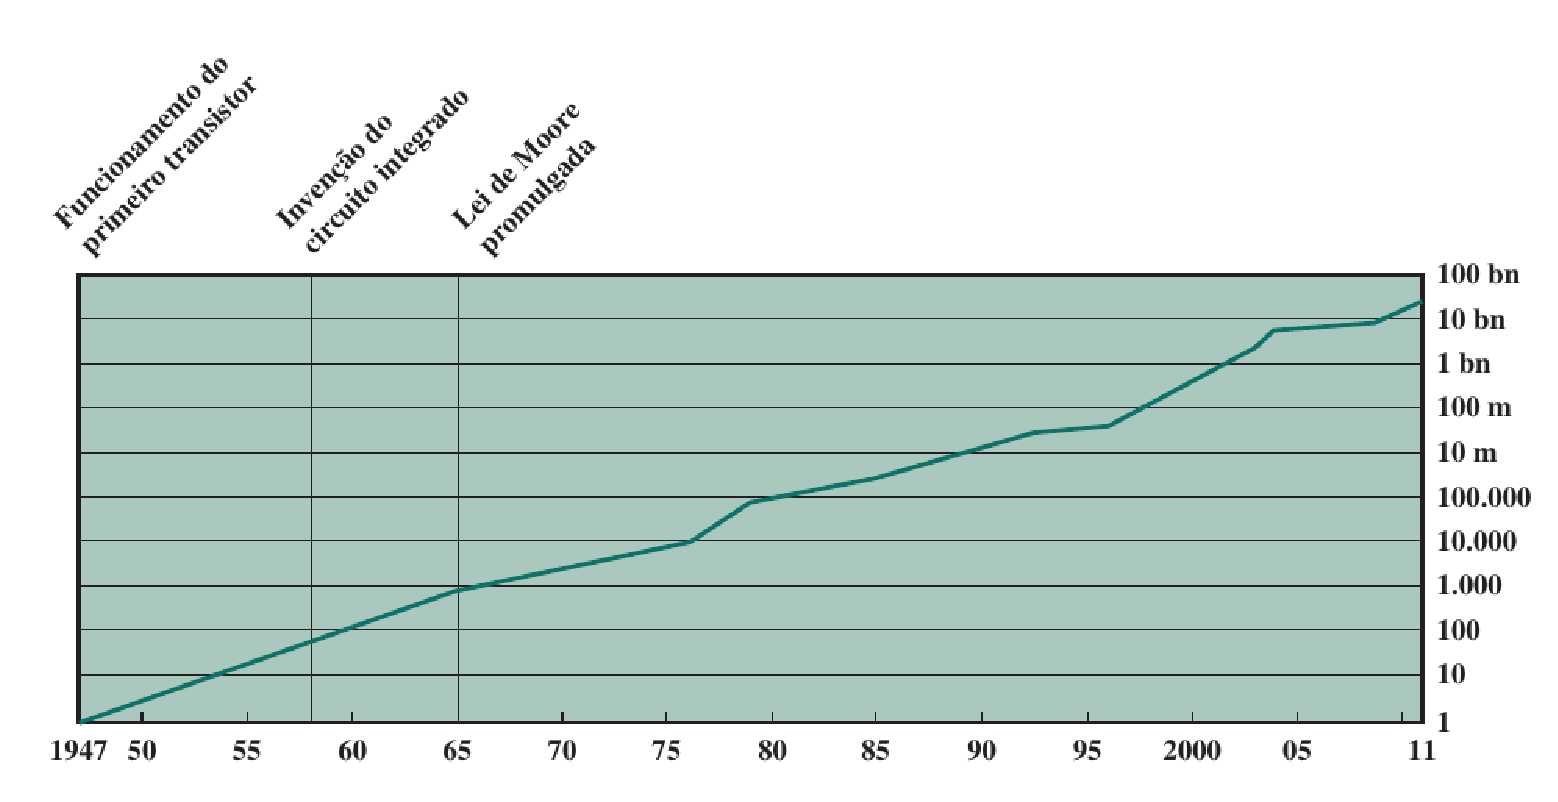
\includegraphics[width=0.8\textwidth]{figs/moore2} 
\end{center}
\end{slide}

%\begin{slide}[toc=]{Consequências da Lei de Moore}
%\begin{itemize}
%\end{itemize}
%\end{slide}



%
\begin{slide}[toc=]{IBM System/360 (1964)}
	\twocolumn{
\begin{itemize}
   \item Substituiu (incompatível com) série 7000
   \item Primeira ``família'' planejada de computadores (mainframes):
	   \begin{itemize}
		   \item Conjuntos de instruções semelhantes ou iguais
		   \item Sistema operacional semelhante ou igual
		   \item Diferentes velocidades, números de portas de E/S, tamanho de memória, e custo (100.000s US\$)
	   \end{itemize}
\end{itemize}}
{Console do IBM 360-65\\
	\includegraphics[width=\textwidth]{figs/IBM360}}
\end{slide}

\begin{slide}[toc=]{Família IBM System/360}
	Modelos da família IBM System/360 e suas características
\begin{center}
   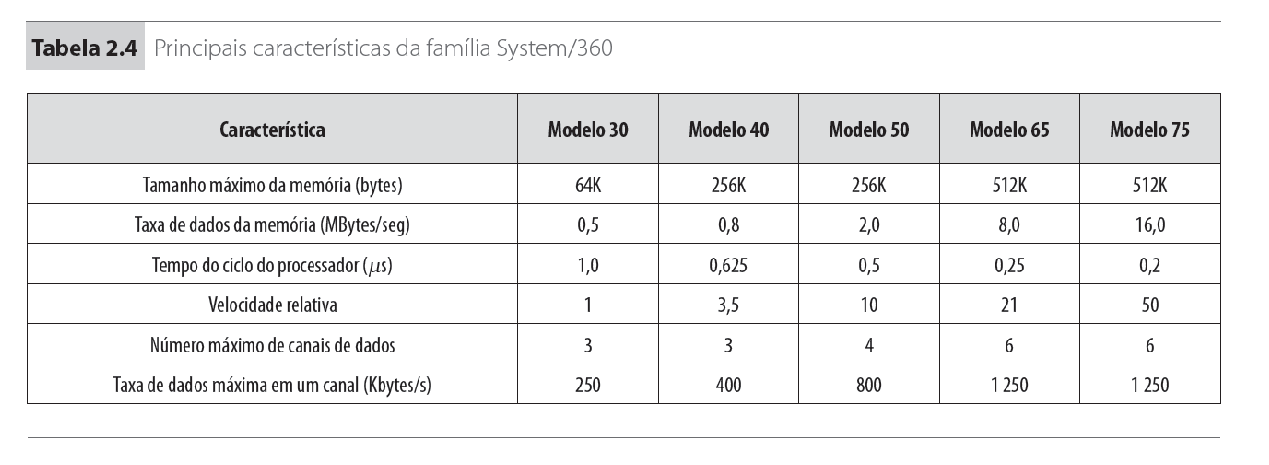
\includegraphics[width=0.99\textwidth]{figs/ibm360} 
\end{center}
\end{slide}

\begin{slide}[toc=]{Digital Equipment Corporation (DEC) PDP-8}
	\twocolumn{
\begin{itemize}
	\item Minicomputador (dava para colocar na bancada do laboratório)
	\item Baixo custo: apenas US\$ 16.000,00 (equivalente a US\$ 150.000,00 em 2019... uma pechincha)
	\item Estrutura de barramento:
		\begin{itemize}
			\item 96 vias (dados, endereços e controle)
			\item Vias compartilhadas
			\item Arquitetura de grande flexibilidade (rever IBM 7094)
		\end{itemize}
\end{itemize}
        \vspace{0.5cm}
	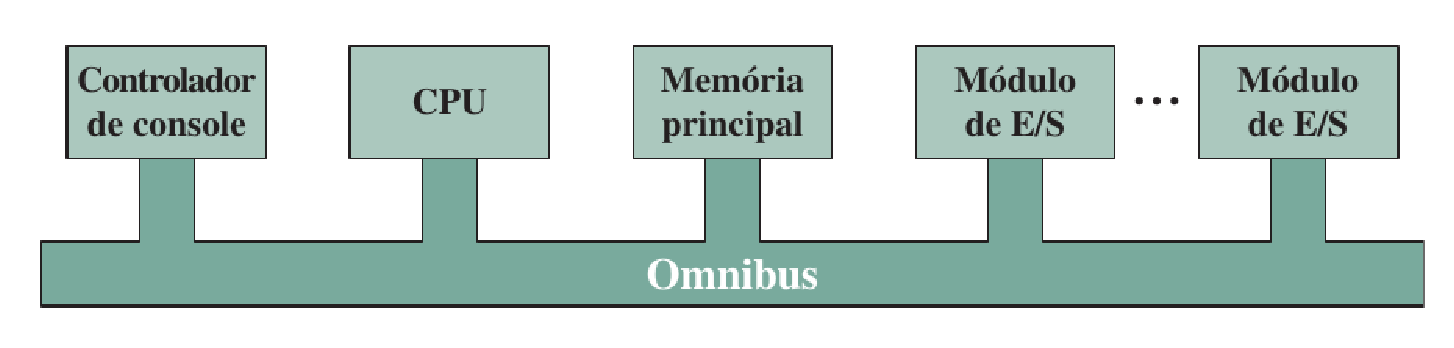
\includegraphics[width=\textwidth]{figs/omnibus}
	}
{Fotografia de um DEC PDP-8
	\begin{center}
	\includegraphics[width=0.6\textwidth]{figs/PDP-8}
	\end{center}}
\end{slide}


\begin{slide}[toc=]{Gerações}
\begin{center}
   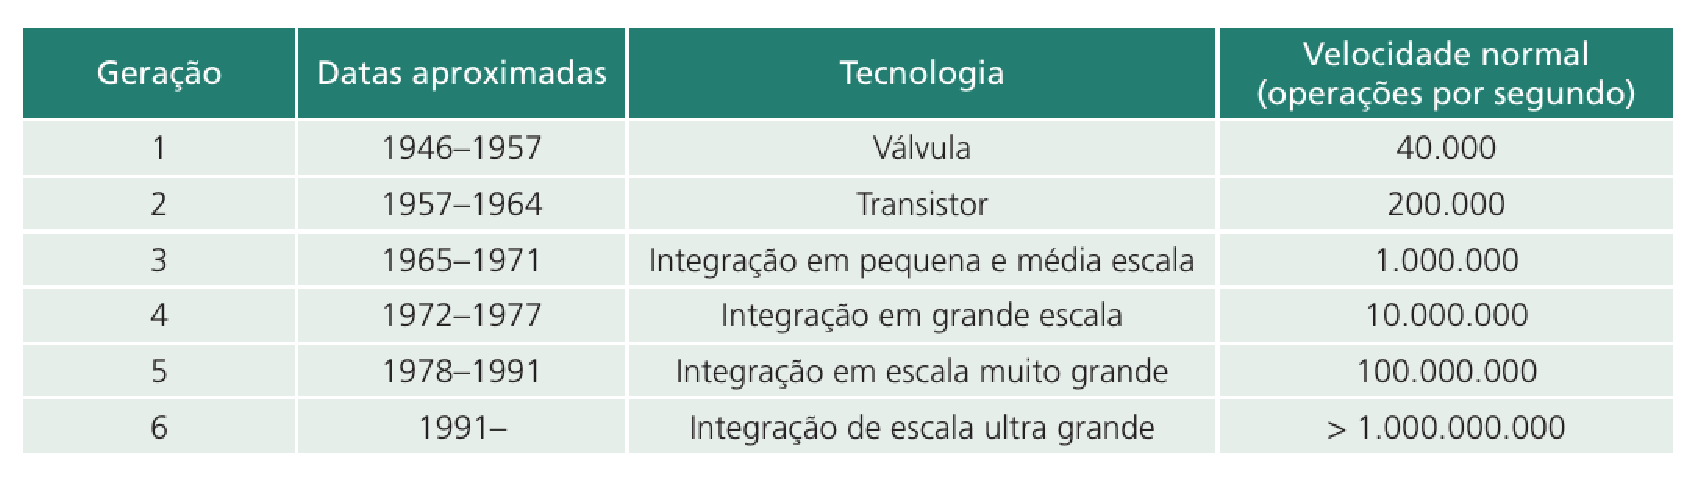
\includegraphics[width=\textwidth]{figs/geracoes2} 
\end{center}
\end{slide}

\begin{slide}[toc=]{Tecnologia de memória}
	\twocolumn{
	\begin{itemize}
		\item Nas décadas de 1950 e 1960, as memórias eram de núcleo magnético
		\item Em 1970, foi construída a primeira memória semicondutora funcional (Fairchild) com capacidade para 256 bits 
		\item Em 1974, o preço do bit da memória semicondutora ficou abaixo do bit da memória de núcleo magnético
	\end{itemize}}
        { Memória de núcleo de Ferrite
	\begin{center} 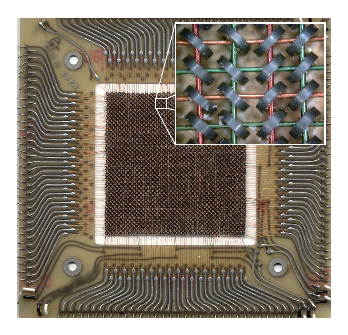
\includegraphics[width = \textwidth]{figs/Ferrite_core_memory}\end{center}}
\end{slide}
%\begin{slide}[toc=]{Processadores Intel - anos 70}
%\begin{itemize}
%   \item 4004: 1971, 108 kHz, 4 bits, 2 300 trans., 640 bytes;
%   \item 8008: 1972, 108 kHz, 8 bits, 3 500 trans., 16 KB;
%   \item 8080: 1974, 2 MHz, 8 bits, 6 000 trans., 64 KB;
%   \item 8086: 1978, 5 (8,10) MHz, 16 bits, 29 000 trans., 1 MB;
%   \item 8088: 1978, 5 (8) MHz, 8 bits, 29 000 trans., 1 MB;
%\end{itemize}
%\end{slide}
%
%\begin{slide}[toc=]{Processadores Intel - anos 80}
%\begin{itemize}
%   \item 80286: 1982, 6-12,5 MHz, 16 bits, 134 000 trans., 16 MB, 1~GB;
%   \item 386TM DX : 1985, 16-33 MHz, 32 bits, 275 000 trans., 4 GB, 64~TB;
%   \item 386TM SX : 1988, 16-33 MHz, 16 bits, 275 000 trans., 16 MB, 64~TB;
%   \item 486TM DX CPU: 1989, 25-50 MHz, 32 bits, 1,2 milhão trans., 4~GB, 64~TB, 8~KB;
%%\end{itemize}
%\end{slide}
%
%\begin{slide}[toc=]{Processadores Intel - anos 90}
%\begin{itemize}
%   \item 486TM SX: 1991, 16-33 MHz, 32 bits, 1,185 milhão trans., 4~GB, 64~TB, 8~KB;
%   \item Pentium: 1993, 60-166 MHz, 32 bits, 3,1 milhões trans., 4 GB, 64~TB, 8~KB;
%   \item Pentium Pro: 1995, 150-200 MHz, 64 bits, 5,5 milhões trans., 64~GB, 64~TB, 512~KB (L1), 1~MB (L2);
%   \item Pentium II: 1997, 200-300 MHz, 64 bits, 7,5 milhões trans., 64~GB, 64~TB, 512~KB (L2);
%\end{itemize}
%\end{slide}
%
%\begin{slide}[toc=]{Processadores Intel - mais recentes}
%\begin{itemize}
%   \item Pentium III: 1999, 450-360 MHz, 64 bits, 9,5 milhões trans., 64~GB, 64~TB, 512~KB (L2);
%   \item Pentium 4: 2000, 1,3-1,8 GHz, 64 bits, 42 milhões trans., 64 GB, 64~TB, 256~KB (L2);
%   \item Core 2 Duo: 2006, 1,06-1,2 GHz, 64 bits, 167 milhões trans., 64 GB, 64~TB, 2~MB (L2);
%   \item Core 2 Quad: 2008, 3 GHz, 64 bits, 820 milhões trans., 64 GB, 64~TB, 6~MB (L2);
%\end{itemize}
%\end{slide}

\end{document}
